\documentclass{article}
\usepackage[UTF8]{ctex}
\usepackage{geometry}
%\usepackage{natbib}
\usepackage{graphicx}
\usepackage{setspace}
\usepackage{caption2}
\usepackage{datetime}
\usepackage{float}

\pagestyle{plain}
\geometry{left=3.18cm,right=3.18cm,top=2.54cm,bottom=2.54cm}

\setmainfont{Times New Roman}
\setCJKmainfont{黑体}

\renewcommand{\today}{\number\year 年 \number\month 月 \number\day 日}
\renewcommand{\captionlabelfont}{\small}
\renewcommand{\captionfont}{\small}

\begin{document}

\begin{figure}
    \centering
    
\includegraphics[width=8cm]{upc.png}
    \label{figupc}
\end{figure}

\begin{center}
	\quad \\
	\quad \\
	\heiti \fontsize{45}{17} \quad \quad \quad
	\vskip 1.5cm
	\heiti \zihao{2} 《计算科学导论》课程总结报告
\end{center}

\vskip 2.0cm
	
\begin{quotation}
	\doublespacing
    \zihao{4}\par\setlength\parindent{7em}
	\quad

	学生姓名:\underline{\quad \qquad \ 尚博文 \ \qquad \quad}

	学\hspace{0.6cm} 号:\underline{\qquad \ 2007010318 \ \qquad}
		
	专业班级:\underline{\qquad \ 计算2003 \ \qquad  }
		
    学\hspace{0.6cm} 院:\underline{计算机科学与技术学院}

	\vskip 2cm
	\centering
	\begin{table}[h]
        \centering
        \zihao{4}
        \begin{tabular}{|c|c|c|c|c|c|c|}
            \hline
            课程认识 & 问题思 考 & 格式规范  & IT工具  & Latex附加  & 总分 & 评阅教师 \\
            30\% & 30\% & 20\% & 20\% & 10\% &  &  \\
            \hline
             & & & & & &\\
             & & & & & &\\
            \hline
        \end{tabular}
    \end{table}
	\vskip 2cm
	\today
\end{quotation}

\thispagestyle{empty}
\newpage

\setcounter{page}{1}

\section{引言}

计算科学导论这门课程,作为计算机科学与技术专业的学科思政课程,从计算科学的历史渊源、学科特点、学科知识体系结构、学科发展规律和趋势等内容,引导学生从科学哲学的角度去认识和学习计算科学,帮助学生更好的认识本科培养方案及培养目标,助力学生建立起对学校“努力构建面向产出的、质量可控的、量化的人才培养体系”的科学合理的认识与分析,使得学生向着成为社会主义合格的建设者和接班人的目标不忘初心,砥砺奋斗。

作为一名计算机科学与技术专业的大一新生,我很荣幸能够听到孙运雷教授为我们带来别开生面的计算科学导论课程。孙教授为我们开启了计算科学的大门,带领我们遨游在计算科学的海洋中,不仅帮助我们拓宽计算科学的视野,而且还帮助我们构建起合理的课程先修关系图及软件研发、网络规划、系统架构、智能应用四个方面的支撑课程。在此,也热烈祝贺我校专业认证的成功,感谢孙老师的努力与付出!

本文将结合我在计算科学领域的学习经历、认识体会等方面,结合课程中对分组演讲城市规划与大数据的探索,分析总结计算科学导论这门课程的重要性及这一阶段的所思所感。希望对自己后续的学习、成长起到启蒙的作用,成为后续不懈奋斗的力量源泉。

\section{对计算科学导论这门课程的认识、体会}

计算科学导论基于计算机学科的计算科学,通过对逻辑结构和经验内容的分析,对科学理论和客观世界关系的分析,对科学理论和科学家关系的分析,帮助我们逐步建立起计算科学的学科方法论和学科方法学。而我国高等院校建设的核心目标就是致力于人才素质的综合培养,对所学专业进行系统化、规范化的建设,使其具有可塑造性和建设性。

计算科学导论这门课程便是如此,它带领大一新生从对计算科学的懵懂到了解,从迷茫到坚定,更加清晰地认识到了当下计算科学发展之机遇,确定自己的目标,追求人生价值的实现。
本节将结合半年来计算科学的学习经验与体会,浅谈计算科学、计算思维和计算人才培养三个方面进行阐述,以彰显计算科学导论这门课程对我在计算科学领域方面的影响,体现计算科学导论对于大一新生的重要性。

\subsection{浅谈计算科学}

计算科学是对描述和变换信息的算法过程,包括其理论、分析、设计、效率分析、实现和应用的系统,是一种新的科学形态。

狭义上,计算科学指的是计算机科学与技术这一一级学科,而广义上,还囊括了计算作为一个学科形态所包含的学术范畴和内涵。自然,研究计算科学,要先研究科学的认识论、科学方法论和科学的逻辑基础。一个科学的认识,一套科学的方法,一套科学的程序,便可以帮助我们探究计算科学哲学,了解计算科学与其他学科的联系,理解计算科学的学科形态、核心概念、典型方法和典型实例。

以数学和电子科学为基础,计算科学是一门理论性、实践性很强的新兴学科,但目前整体上对计算科学的理论研究仍然滞后于技术开发。举例来说,当下对于芯片制造行业来说,深究5nm工艺背后的理论支持或许并不那么容易,但是参照经验科学的工作方式却可能将其规模量产。计算科学并不完全排斥经验科学,但是单纯靠经验科学来发展一门学科,是极其不稳定的。

社会的广泛应用需求推动了计算科学的发展,新一代信息技术产业大都与计算科学的发展密切相关。5G、新型电子元器件、集成电路设计制造、量子计算机……计算科学正帮助人类突破一道又一道技术难关,更好的服务于社会,贡献于世界。

\subsection{浅谈计算思维}

计算思维是一种重要的思维方式\cite{ref1}。它最早由麻省理工学院的Seymour Papert教授提出\cite{ref2},并由卡内基梅隆大学的周以真教授推广\cite{ref3}。对于计算思维的理解和应用,具有极为重要的意义。

计算思维能够帮助我们将一个具体的问题抽象化,进而形成能让计算机“理解”的可计算模型,并且在有限的时空内得出结果。它在专业能力和信息素质培养上的重要性是不言而喻的。它不仅是把现实问题变成计算机可计算模型并产生结果的思维过程,而且它与计算实践密切相关。

众所周知,计算科学拥有着悠久的数学起源。从丢番图方程到可计算性问题,一次又一次数学危机引导人们不断探索计算科学之哲学思想。哥德尔的不完备定理的出现,使得许多数学家试图将可计算性理论形式化,一般递归函数、λ算子、图灵机便是其中典型的代表。而随着计算科学的发展,计算思维也随之形成。

随着计算机智能化程度的提升和计算能力的不断增强,人类对于世间万物的认知,对于复杂算术的运算,对于抽象问题的解决,都是人类计算思维的综合体现。伴随着计算实践,计算思维才能服务于设计和构造,才能帮助人们认识、研究和改造世界,进而促进社会的进步。

因此,没有计算实践而空谈计算思维是没有意义的,我们自然而然也无法感觉到程序的美感。当然,无论我们未来是否从事与计算科学相关的工作,这种将一个大问题分解为若干个子问题的自顶向下的结构化设计方法会充斥在我们的日常生活中,帮助我们处理生活的琐事,更加清晰的认识世界和改变世界。

\subsection{浅谈计算人才培养}

近年来,中美贸易摩擦的不断升级和美国在芯片产业上对中国的封锁,极大的震撼了中国的产业界,这也为计算人才的培养敲响了警钟。

《教育部关于深化本科教育教学改革全面提高人才培养质量的意见》\cite{ref4}指出,要进一步指定个性化的培养方案和学业生涯规划,推进模块化课程建设,丰富优质课程资源,进一步激励学生刻苦学习,引导学生爱国、励志、求真、力行。

我校计算机科学系“努力构建面向产出的、质量可控的、量化的人才培养体系” \cite{ref5},帮助国家培养适应新时代信息化、网络化、智能化深度驱动社会主义现代化发展需要,能够在计算应用及相关领域从事软件研发、网络规划、系统架构或智能应用等工作的工程技术人才,帮助学生培养问题分析、分析开发方案、研究与设计等能力,不仅帮助学生培养了计算思维,培养了基本的技能,而且鼓励学生的个性化发展,在四个发展方向上开拓思维,锻炼能力,提升学生的综合素质和专项能力。

我相信,在共和国纲领性文件的指导下,在学校的培养下,在计算机科学系老师们辛勤的付出下,越来越多的计算人才将不断涌现,终为我国培养出德智体美劳全面发展的社会主义建设者和接班人。

\section{进一步的思考}

\subsection{城市规划与大数据}

随着科学技术水平的不断发展,城市化进程不断加快,智慧城市成为当前城市的主要发展方向,为进一步推动智慧城市发展,解决智慧城市规划中存在的多种问题,需要应用大数据技术。

\subsubsection{城市规划基本知识}

通过对书籍《城市规划概论》\cite{ref6}的阅读,我了解到城市规划、风景园林、土木建筑、环境艺术、环境工程、公共管理等专业及相近、相关专业知识,设计城市形式与发展、城市规划的基本概念、工作内容、制定与实施管理及术语等。通过对本课程的学习,我对城市规划工作有了一个基本的、全面的认识和了解。城市规划是为了实现一定时期内城市的经济和社会发展目标,确定城市性质、规模和发展方向,合理利用城市土地,协调城市空间布局和各项建设所作的综合部署和具体安排

\subsubsection{大数据的特点}

通过视频以及查看书籍,我了解到:大数据主要是对大量数据的对比,对相同类型或者不同方面的数据进行计算,归纳相关事物的特点,明确不同事物之间的联系性,实现对事物发展的有效推算,并作出预测,为事物或社会的发展提供方向。大数据有很多优点,首先,对大量数据的有效收集能力,可以保证相关推算的准确性。其次,种类的多样性,能够实现对多个不同方面事物的推算。再次,大数据的处理速度较快,与普通算法相比,大数据可提升相关推算工作的效率。由于数据量的冗杂,因此,大数据的价值密度相对较低,价值却很高。最后,大数据真实性高,推算结果准确,推算错误问题较少出现。

\subsubsection{大数据与智慧城市}

在智慧城市的规划建设中,大数据具有对城市相关数据信息进行智慧化处理的能力。通过对大数据在城市建设不同领域中的应用,能够为相关领域的决策提供充足的支撑作用。在城市管理中,城市的合理规划和城市的科学管理需要应用大数据技术的运算能力,保障城市的自动化发展。因此,在智慧城市规划建设中,要建立完善的大数据分析中心,收集城市大量的数据,但要确保数据的真实性,保证大数据分析结果的正确性。在智慧城市规划建设中,要有相应的部门保证大数据应用工作的常态化,保证智慧城市管理工作的高效运行。在地方城市层面的应用过程中,可以建立相关部门、地方与企业三方合作模式,更加充分发挥大数据的优势,激发城市更大的商业价值,推动智慧城市的进一步发展。

\subsubsection{城市空间规划中大数据的应用}

在阅读知网论文《洗尽铅华 返本还原——手机大数据在城市规划、交通分析与城市管理中的应用》\cite{ref7}之后,我又了解到:规划智慧城市过程中,需要应用多规协同体系,这一体系在实际应用中则需要运用大量的数据,因此,为有效完善智慧城市的规划建设,需要应用大数据技术。在多规协同体系中,大数据的实际应用要对城市整体的发展情况进行分析,在建设智慧城市的过程中,可以充分应用大数据技术,促进城市不同领域之间的协同发展,使整个协同体系更加智能化。

城市的传统规划方式中,涉及的城市部门相对较多,其中城市行政管理部门对城市的整体规划有较大的影响。因此,要保障城市整体规划效果,进一步提升城市行政管理能力和水平。智慧城市规划中,需要充分考虑城市行政管理内容的多样性,应用大数据技术明确规划体系,确定规划内容,加强对数据信息的保护,提升智慧城市规划质量。多规协同体系中大数据的应用,要注意避免重复使用数据,应结合智慧城市的规划要求确定相应的建设策略,保证相关策略的有效应用。多规协同体系的构建基础是大数据技术,应用大数据技术才能更好完善多规协同体系,促进智慧城市空间规划的规范化发展。同时,大数据技术能够为城市环保化与智能化发展提供相应的指导建议,对于城市资源的有效分配、发挥智慧城市价值有重要的作用。智慧城市应用大数据技术整合城市信息,推动智慧城市的建设发展,对智慧城市多规协同体系的建设与发展有支撑作用,对智慧城市的发展有较大的推动作用。

\subsection{对于大数据的个人思考}

我认为,所谓的“大数据”其实是包含两个方面,一个是数据,另一个就是大。

在大数据这个概念出来之前的数据指的是实验数据、统计数据等,就是一个数字的形式表现出来;也可能是信息和情报等;作为程序员提到数据更多指的是数据库中的数据。

数据量在没有出现大容量的存储空间和自动化的处理计算机之前是很小的。纸质的表格文件,既不容易记录整理也不容易存储,在整理和归类过程中的需要花费巨大的人力,而且还不一定保证数据的准确性。

随着计算机的计算能力的提高和存储空间的扩大人们现在存储的数据形式和数据量都有了很大的改观。存储的数据形式也不再是单一的表格数据,而扩展成声音、图片、视屏等多种多样的数据格式。

每个人都有属于自己的格式,重要的数据包括:身份证号、姓名、性别、所在城市、居住地址、工作单位、手机号码等属于个人隐私的数据,其他数据还有所开的汽车、家庭收入、孩子的学校、日常开支等,再者就是经常出入的场所、爱吃的餐厅、经常逛的网页等。这些数据在多个维度上展现了一个人的情况。也许有人会觉得除了隐私的一些数据之外其他的数据即使别人知道了也无所谓。一个人的一些数据被知道也无所谓,但是一旦这个人的其他一些数据同时被知道了,那么就可以通过这些数据分析出这个人当前的一些具体情况。这也就是为什么购物网站经常会推送给你一些你可能会需要的东西。

对于一些数据,有人觉得可以通过统计的形式获得,但是这里面执行的难度就很大了。首先要设计合理的问卷,然后在针对不同的人群选择不同年龄段,还要选择不同的地区。最后统计完成之后,如果发现统计维度少了一个,如果再增加一个维度的话,相当于重新再做一次调查,成本几乎就和上一个调查一样。

还有一个很重要的原因,就是人们通过问卷调查填写的数据未必就是大家心里真实的想法。有些人为了使自己显得不是很另类或者让自己显得有面子,通常会填写一些高大上的答案。而人们在网络上填写的数据是不会有压力的,因为都是匿名的,没有人知道你是谁,没有人关心你的姓名,人们只是知道有这么个人发表了这样或者那样的言论或者答案等。

大数据的重要性在于它的多维度和完备性。

过去人们统计的数据依赖于计算能了和存储空间,包括问卷调查,因此收集数据只会收集到有限的几个维度的数据,其他维度的数据就被自动的忽略掉了。
大数据可以从数据的本身出发,不带有任何想法和偏见,看看数据本身能够带来什么样的结论。

无论在什么领域,或者从事什么行业,谁懂得数据的重要性,谁会在工作中善于利用数据,谁就用可能会更成功!

\section{总结}

时光荏苒,岁月如梭,半年大学生活转瞬即逝。在孙运雷教授的指导下,我了解到了计算科学的发展历程,认识到了计算科学未来的发展方向,感受到了计算科学导论这门课程的重要性。

我知道,计算科学导论只是引导我们去了解计算科学下的诸多分支,帮助我们浅显的认识分支学科所包含的内容及其未来可能的发展方向,帮助我们更好的度过大一迷茫的生活,桥接高中与大学,帮助我们更清晰的认识到计算科学发展现状,引导我们认识问题、思考问题,尝试给出可能的解决方案,锻炼我们的基本素质。

未来,我将不负韶华,以更加饱满的精力,更加坚定的决心,更加顽强的毅力,更加努力的探索,在计算科学导论所建成的总体框架下,不忘初心,认真学习科学文化知识,全面提高自身综合素质,向着成为一名网络安全方面人才不断前行,向着成为社会主义事业合格的建设者和接班人不懈奋斗。

\section{附录}

\subsection{Github}

个人网址:https://github.com/SummerWind18

截图:
\begin{figure}[H]
    \centering
    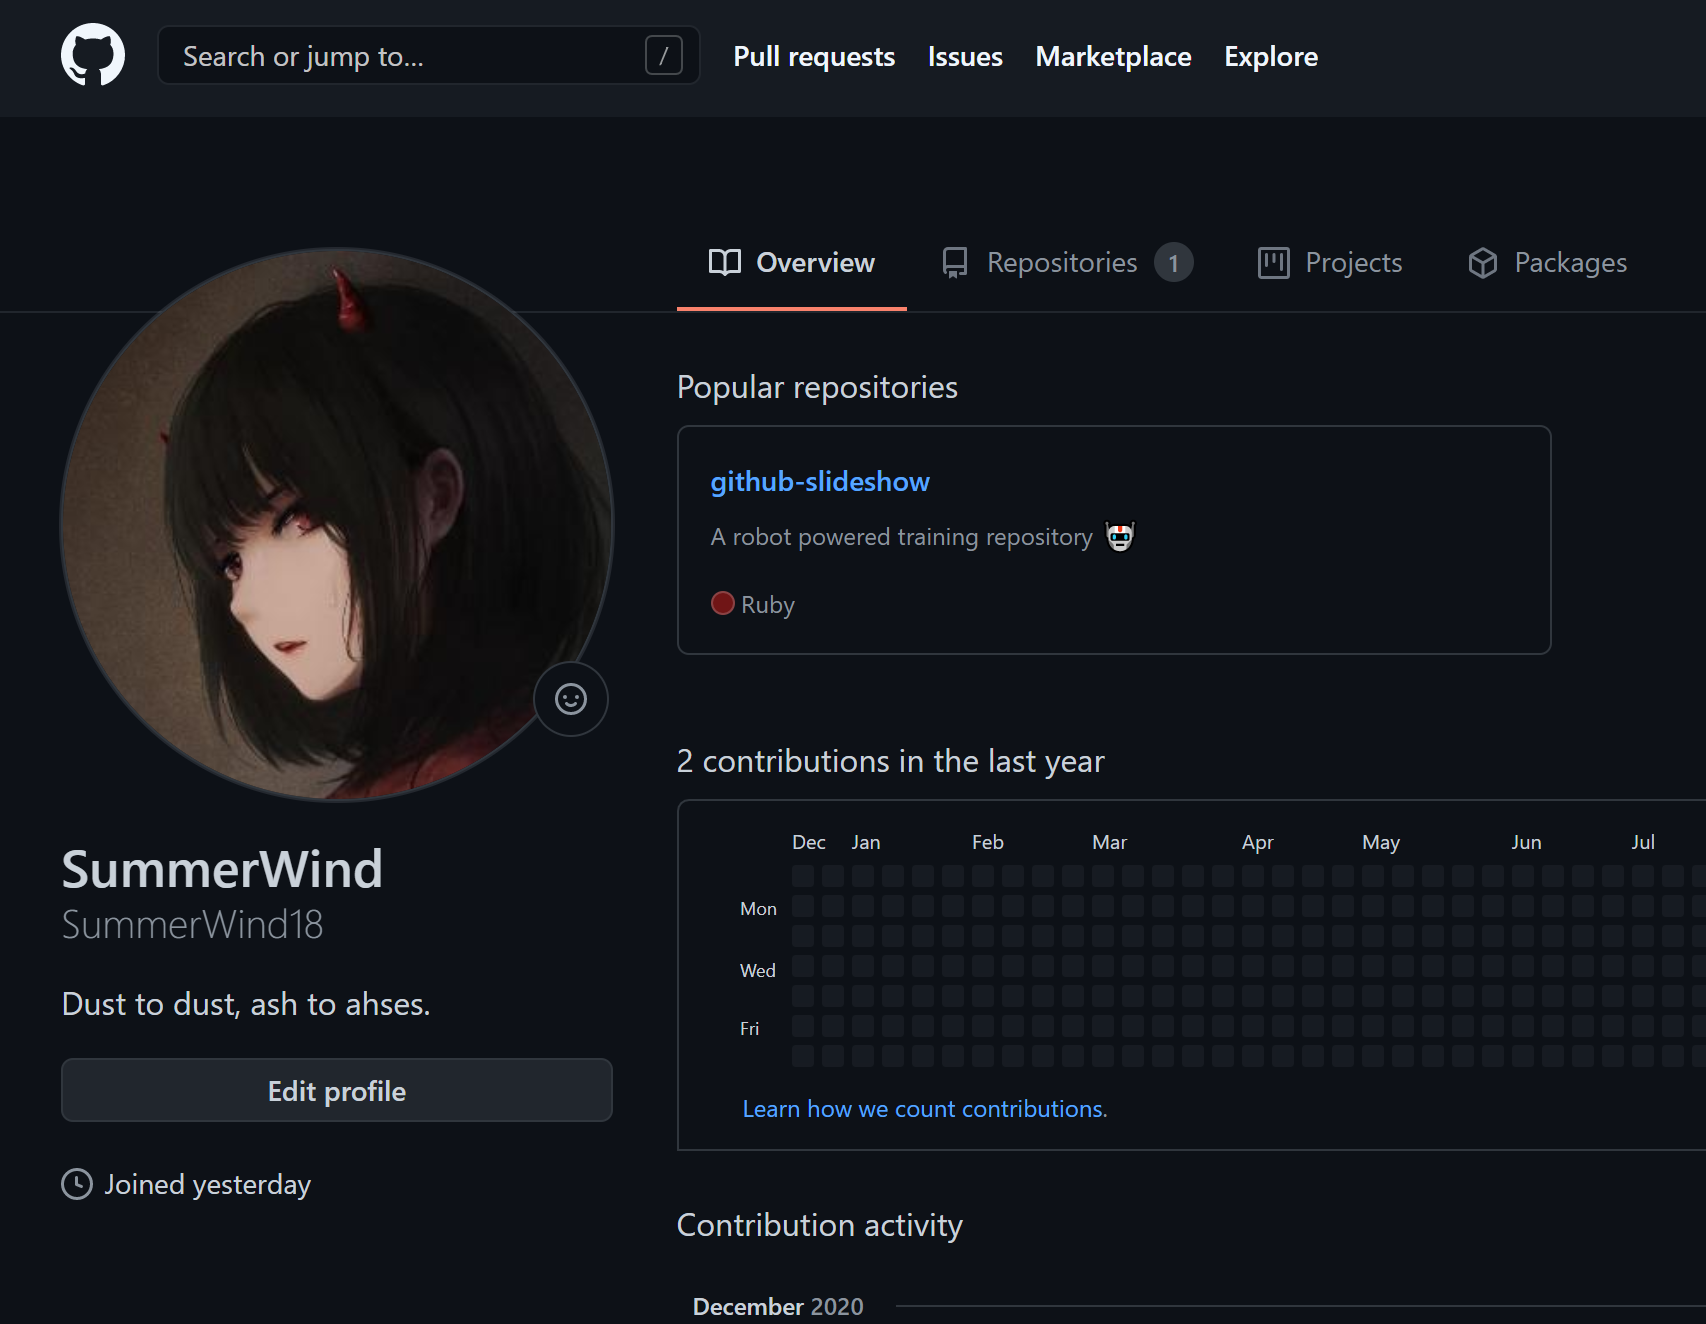
\includegraphics[scale=0.3]{Github}
    \label{fig:Github}
\end{figure}

\subsection{观察者}

截图:
\begin{figure}[H]
    \centering
    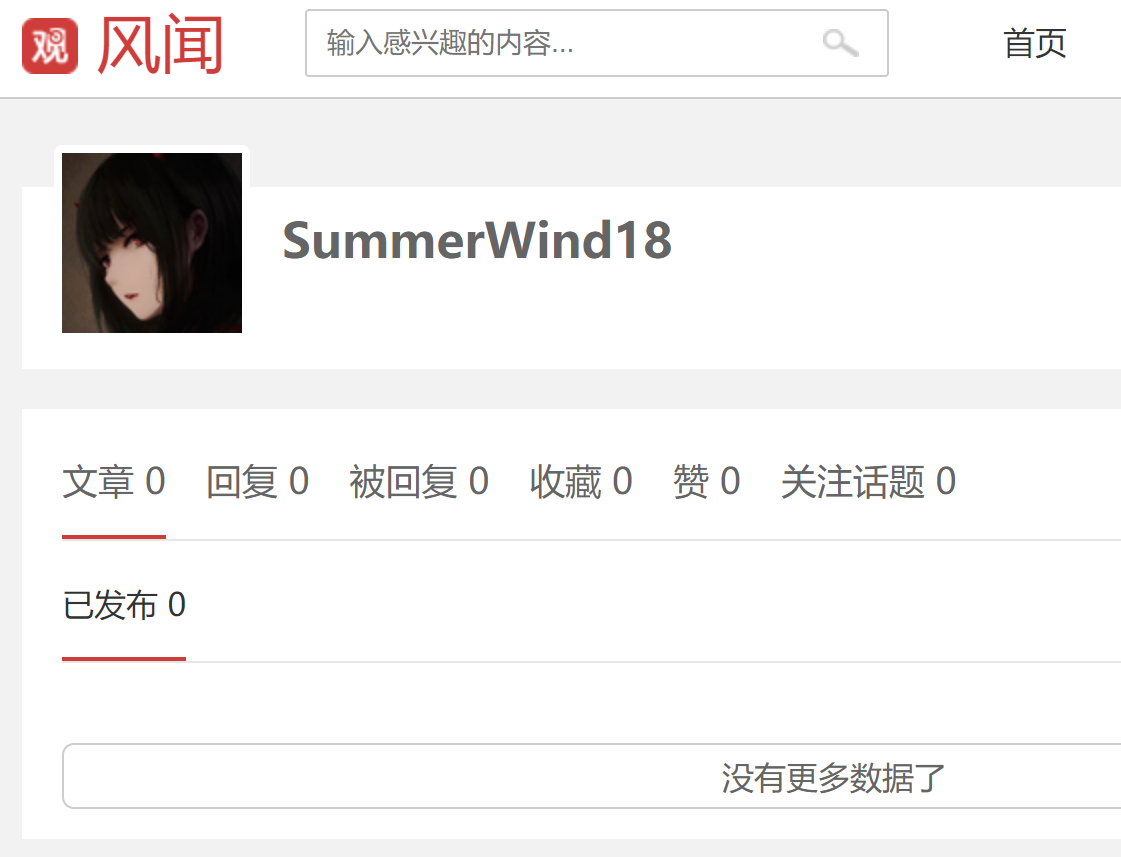
\includegraphics[scale=0.28]{gcz}
    \label{fig:gcz}
\end{figure}

\subsection{学习强国}

截图:
\begin{figure}[H]
    \centering
    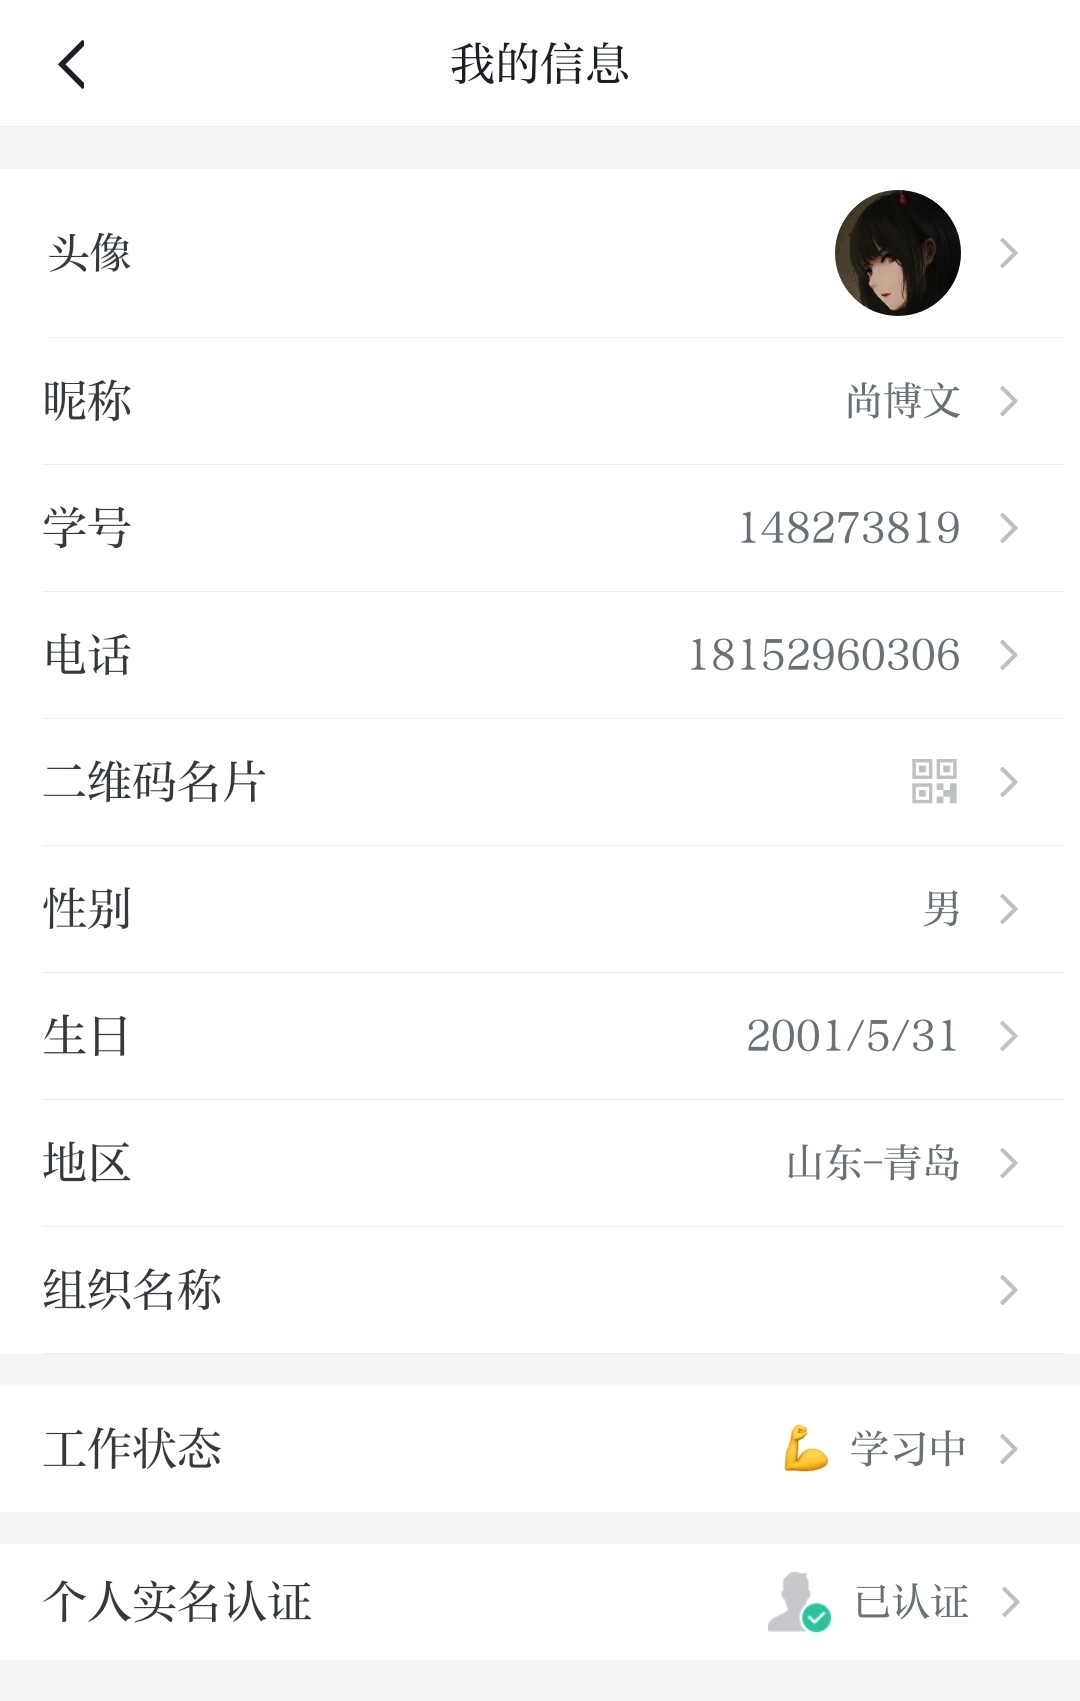
\includegraphics[scale=0.28]{xxqg}
    \label{fig:xxqg}
\end{figure}

\subsection{哔哩哔哩}

截图:
\begin{figure}[H]
    \centering
    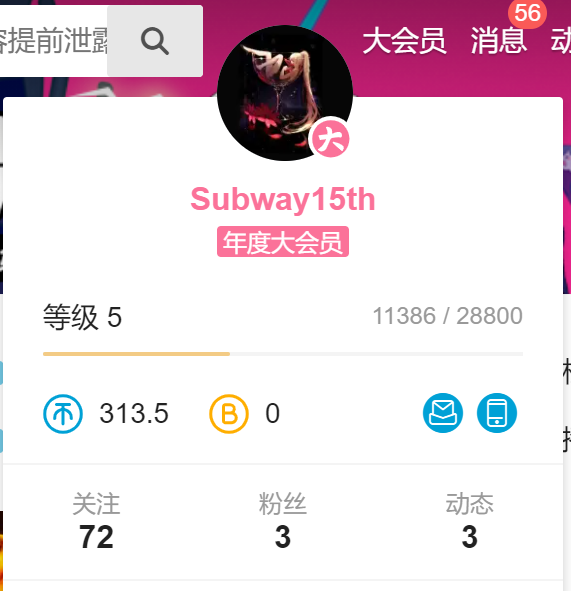
\includegraphics[scale=0.28]{Bilibili}
    \label{fig:Bilibili}
\end{figure}

\subsection{CSDN}

个人网址:https://blog.csdn.net/Subway18

截图:
\begin{figure}[H]
    \centering
    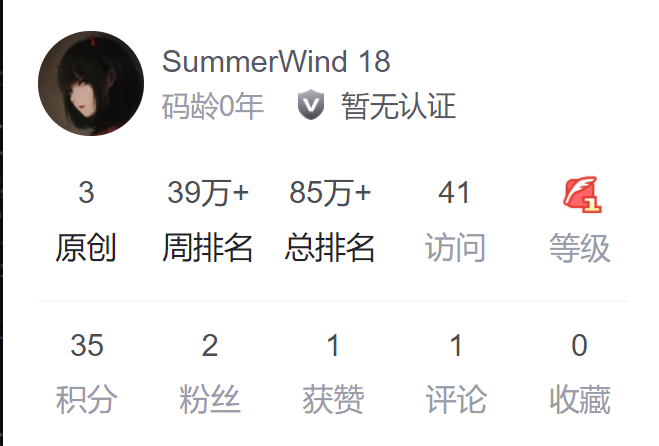
\includegraphics[scale=0.5]{CSDN}
    \label{fig:CSDN}
\end{figure}

\subsection{博客园}

个人网址:https://home.cnblogs.com/u/2260781/

截图:
\begin{figure}[H]
    \centering
    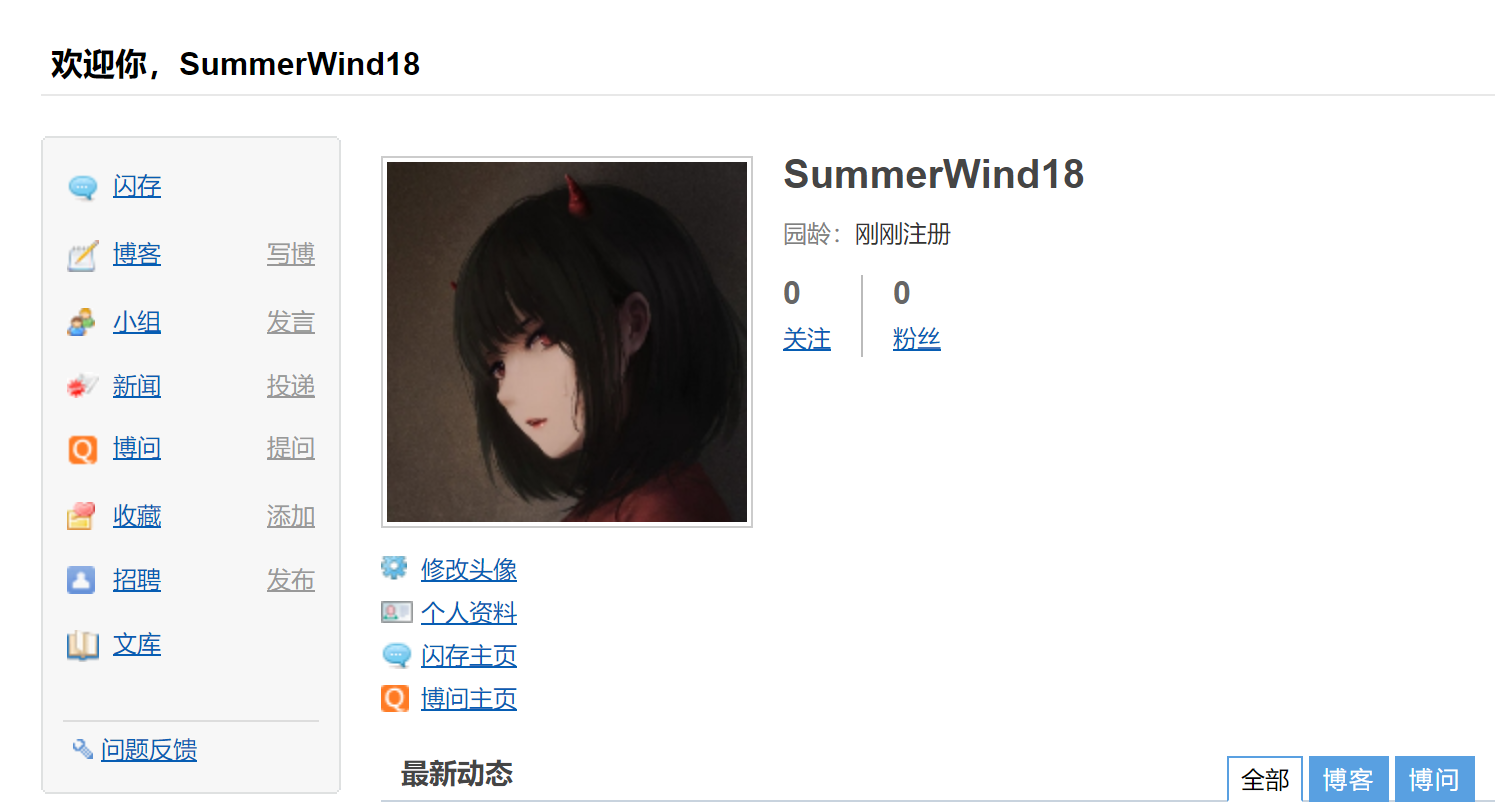
\includegraphics[scale=0.5]{blog}
    \label{fig:blog}
\end{figure}

\subsection{小木虫}

个人网址:http://muchong.com/bbs/space.php?uid=24814531

截图:
\begin{figure}[H]
    \centering
    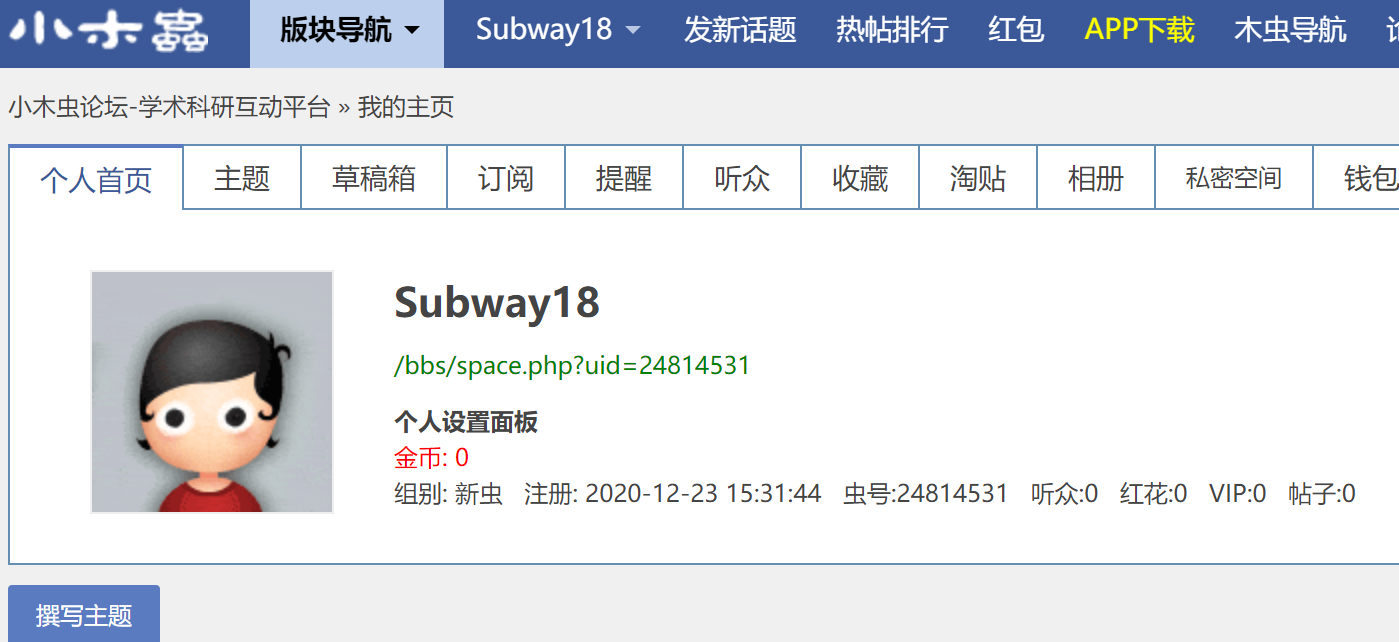
\includegraphics[scale=0.5]{xmc}
    \label{fig:xmc}
\end{figure}

\begin{thebibliography}{9}
    \bibitem{ref1} 杜子徳. 计算思维及其意义. 中国计算机学会通讯, 2019, 10
    \bibitem{ref2} Seymour Papert. An Exploration in the Space of Mathematics Educations[J]. International Journal of Computers for Mathematical Learning, 1996, (1): 95-123.
    \bibitem{ref3} Jeannette M. Wing. Computational Thinking[J]. Communications of the ACM, 2006, (3): 33-35
    \bibitem{ref4} 中华人民共和国教育部. 关于深化本科教育教学改革全面提高人才培养质量的意见. [2020-1-1]. moe.gov.cn/srcsite/A08/s7056/201910/t20191011\_402759.html
    \bibitem{ref5} 中国石油大学(华东)计算机科学与技术学院. 计算机科学与技术专业-工程教育认证. [2020-1-1]. ceea.upc.edu.cn
    \bibitem{ref6} 陈锦富.城市规划概论. 中国建筑工业出版社, 2006
    \bibitem{ref7} 洗尽铅华 返本还原——手机大数据在城市规划、交通分析与城市管理中的应用. 邹亚华 2016.12

\end{thebibliography}


\end{document}
